\documentclass{article}
\usepackage[utf8]{inputenc}
\usepackage{enumerate}
\usepackage{enumitem}
\usepackage{float}
\usepackage{graphicx}
\usepackage{multirow, array}
\usepackage[spanish,activeacute]{babel}


\title{Práctica 3: Gestión de una Web de cine}
\author{Rafael Nogales Vaquero
\\Lothar Soto Palma
\\Elena Toro Pérez
\\Jose Ramón Trillo Vilchez}
\date{\today}

\begin{document}
\maketitle

\section{Diagramas de Conceptos}
	\subsection*{Gestión de usuarios. \textit{Elena Toro Pérez}}
		\textbf{Problema:} Los \textbf{administradores} necesitan mantener un control en los \textbf{usuarios} del sistema.
Los \textbf{usuarios registrados} deberán identificarse y podrán darse de alta o de baja en registro.\\
\textbf{Conceptos:} Administrador, Usuario, Usuario Registrado.\\
\textbf{	Relaciones:}
	\begin{itemize}
    	\item El administrador controla los usuarios del sistema.
        \item El administrador gestiona los usuarios registrados en el sistema.
        \item Los usuarios, al darse de alta, pasan a formar parte de los usuarios registrados en el sistema.      	
    \end{itemize}
	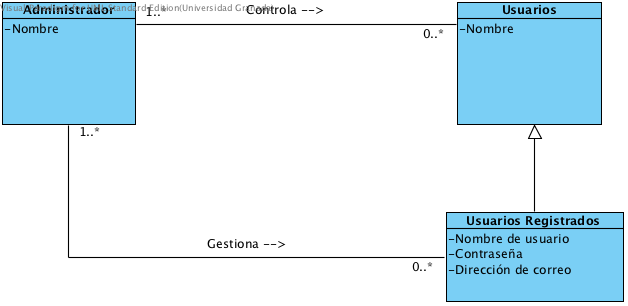
\includegraphics[width=1\linewidth]{./C-Usuarios}


	%Rafa Nogales
	\subsection*{Gestión de películas. \textit{Rafael Nogales Vaquero}}
	\textbf{Problema:} Los \textbf{administradores} necesitan mantener un orden en las \textbf{películas} del sistema.
	 Tan solo los \textbf{usuarios VIP} podrán añadir películas.\\
	\textbf{Conceptos:} Administrador, Usuario VIP, Solicitudes de añadir Películas, Películas.\\
	\textbf{	Relaciones:}
		\begin{itemize}
			\item Los administradores añaden distribuciones de peliculas.
			\item Todos los usuarios (incluídos los administradores) consultan películas.
			\item Los administradores añaden estrenos de películas.
			\item Los administradores añaden premios de películas.
			\item Los administradores añaden trailers de películas.
			\item Los VIP pueden añadir películas y los administradores aceptar o denegar las solicitudes.		
		\end{itemize}
	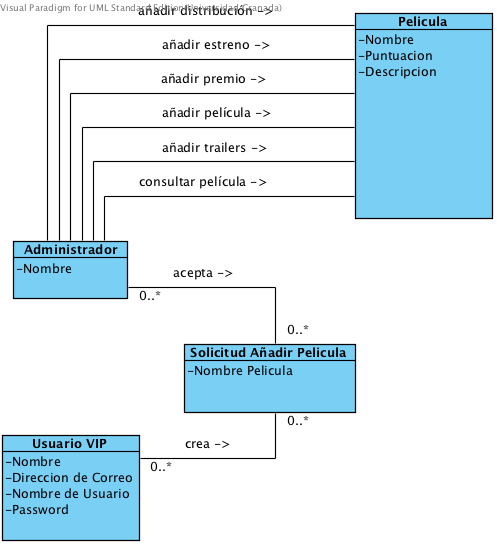
\includegraphics[width=0.7\linewidth]{./C-GestionDePeliculas}
	
	
	%Rafa Nogales
	\subsection*{Gestión de cartelera. \textit{Rafael Nogales Vaquero}}
	\textbf{Problema:} Los \textbf{administradores} necesitan administrar los \textbf{cines} del sistema para saber en que horarios se proyectan 
	las \textbf{películas} en cada cine (\textbf{Programación}).
	\textbf{Conceptos:} Administrador, Cine, Programación, Películas.\\
	\textbf{	Relaciones:}
		\begin{itemize}
			\item Los administradores consultan la programación de las películas.
			\item Los administradores modifican la programación de las películas.
			\item Los administradores dan de alta las programaciones de las películas.
			\item Los administradores dan de alta cines.
			\item Los administradores dan de baja cines.
		\end{itemize}
	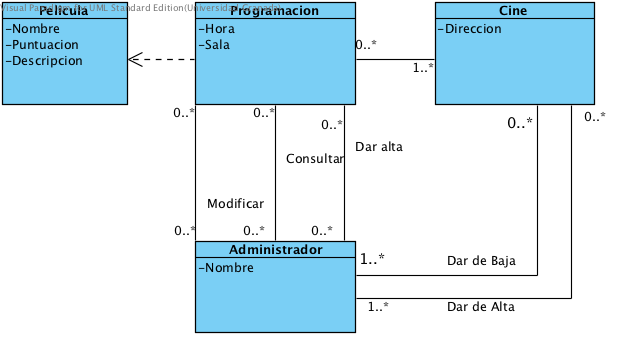
\includegraphics[width=1\linewidth]{./C-Cartelera}
		
	\subsection*{Gestión de Perfil. \textit{Jose Ramón Trillo Vilchez}}
	\textbf{Problema:} Los \textbf{usuario registrado} necesita gestionar la información que le muesta al sistema.
El \textbf{temporizador} se encarga que en un tiempo determinado se busque una cantidad de posibles almas gemelas\\
\textbf{Conceptos:} Temporizador, Usuario Registrado.\\
\textbf{	Relaciones:}
	\begin{itemize}
    	\item El temporizador determina el tiempo que tiene un buscador de encontrar posibles almas gemelas para que luego se muestren a los usuarios.      	
    \end{itemize}
    		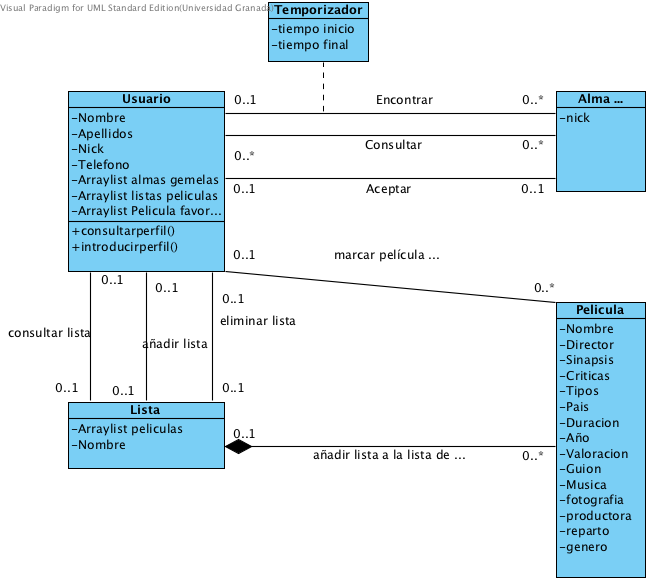
\includegraphics[width=1\linewidth]{./C-Perfil}

	%Lothar Soto
	\subsection*{Gestión de películas por usuarios. \textit{Lothar Soto Palma}}
	\textbf{Problema:} Los \textbf{usuarios} podrán buscar \textbf{películas} en el sistema además de consultar la \textbf{cartelera} de \textbf{Cines}, solo si están \textbf{registrados} podrán puntuarla y tan solo los \textbf{usuarios VIP} podrán añadir y criticar películas.\\
	\textbf{Conceptos:} Usuario, Usuario registrado, Usuario VIP, Cines, Películas, Cartelera.\\
\textbf{	Relaciones:}
		\begin{itemize}
			\item Un cine tiene una cartelera.
			\item Todos los usuarios buscan películas.
			\item Todos los usuarios consultan la cartelera.
			\item Los registrados y los VIP pueden puntuar las películas.
			\item Los VIP pueden criticar y añadir películas.		
		\end{itemize}
			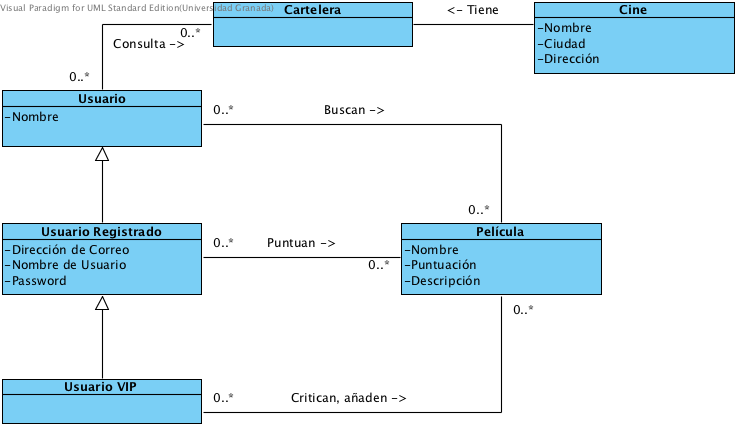
\includegraphics[width=1\linewidth]{./C-PeliculasUsuarios}
	
	%Lothar Soto	
	\subsection*{Gestión de comunidades. \textit{Lothar Soto Palma}}
	\textbf{Problema:} Un \textbf{usuario registrado} se va a encargar de crear \textbf{comunidades} y consultarlas. Los \textbf{usuarios} pueden pedir ser \textbf{miembro} de una \textbf{comunidad}, y si son \textbf{dueños} de una de ellas admitir otros \textbf{usuarios} en ellas. Por último pueden listar \textbf{películas} criticadas por una \textbf{comunidad} o anádidas por la misma.\\
	\textbf{Conceptos:} Usuario registrado, Comunidades, Miembro, Dueño.
	\textbf{Relaciones:}
		\begin{itemize}
			\item Los usuarios crean comunidades.
			\item Los usuarios consultan comunidades.
			\item Los usuarios son miembros de otras comunidades.
			\item Los usuarios son dueños de comunidades.
			\item Los usuarios pueden listar películas.
			\item Las películas pueden ser criticadas por la comunidad.
			\item Las películas pueden ser añadidas por la comunidad.
		\end{itemize}
		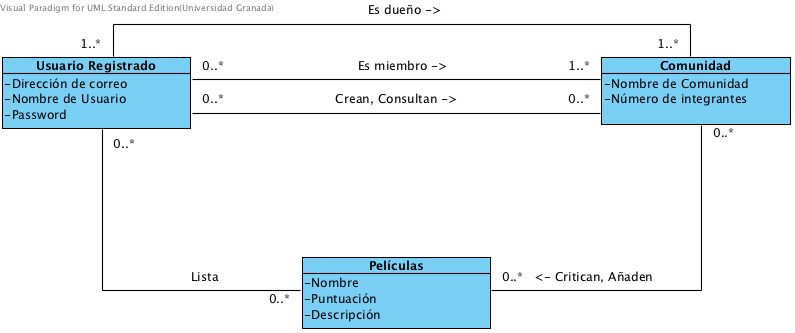
\includegraphics[width=1\linewidth]{./C-Comunidades}
		
\section{Diagramas de Secuencia}
	\subsection*{Gestión de usuarios. \textit{Elena Toro Pérez}}
		\begin{enumerate}
			\item El administrador puede dar de baja a un usuario.
    			\item El administrador puede consultar la información de un usuario.
    			\item El administrador puede pasar un usuario a VIP.
    			\item Un usuario registrado tiene la obligación de identificarse.
    			\item Un usuario registrado puede darse de alta en registro.
    			\item Un usuario registrado puede darse de baja en registro.
		\end{enumerate}
		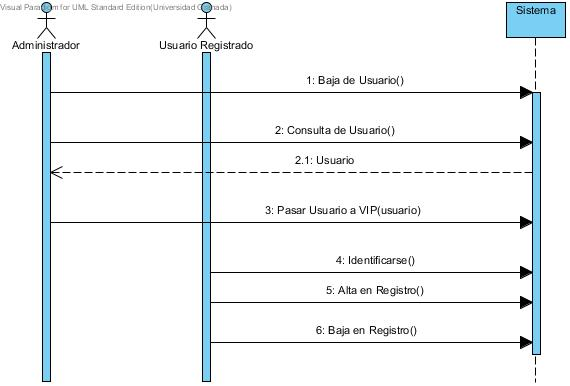
\includegraphics[width=1\linewidth]{./S-Usuarios}
	\subsection*{Gestión de películas. \textit{Elena Toro Pérez}}
		\begin{enumerate}
   	 		\item El Administrador puede aceptar una película añadida por un usuario VIP.
   		    \item El Administrador puede añadir una distribución de una película.
        		\item El Administrador puede añadir en el sistema el estreno de una película.
        		\item El Administrador puede añadirle un premio a una película.
        		\item El Administrador puede añadir una película en el sistema.
        		\item El Administrador puede añadirle los trailers a una película.
        		\item El Administrador puede consultar una película para obtener su información.
    		\end{enumerate}
    		\includegraphics[width=1\linewidth]{./S-peliculas}
	\subsection*{Gestión de cartelera. \textit{Rafael Nogales Vaquero}}
	\begin{enumerate}
		\item El administrador registra un cine en el sistema.
		\item El administrador puede dar de alta la programación de una película en algún cine.
		\item El administrador puede modificar las programaciones de las películas.
		\item El administrador puede consultar la programación de las películas (como el resto de usuarios).
		\item El administrador puede eliminar cines del sisitema.
	\end{enumerate}
			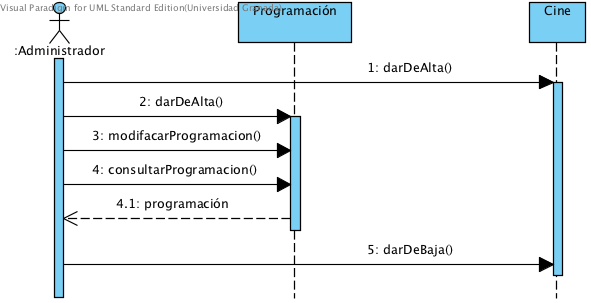
\includegraphics[width=1\linewidth]{./Sec-Cartelera}

	\subsection*{Gestión de Perfil. \textit{Jose Ramón Trillo Vilchez}}
	\begin{enumerate}
		\item El usuario registrado debe de meter datos en su perfil.
    		\item El usuario registrado puede consultar su información.
    		\item El usuario registrado puede marcar una película como favorita.
    		\item Un usuario registrado puede aceptar alguna alma gemela de las candidatas.
    		\item Un usuario registrado puede consultar la lista de sus almas gemelas.
    		\item Un usuario registrado puede añadir una lista de películas personal.
    		\item el usuario registrado puede consultar la lista de películas
    		\item el usuario regustrado puede eliminar una lista de películas
    		\item el usuario registrado puede añadir una película a una lista de peluculas
    		\item el temporizador deber poner un limite a la hora de encontrar almas gemelas
	\end{enumerate}
	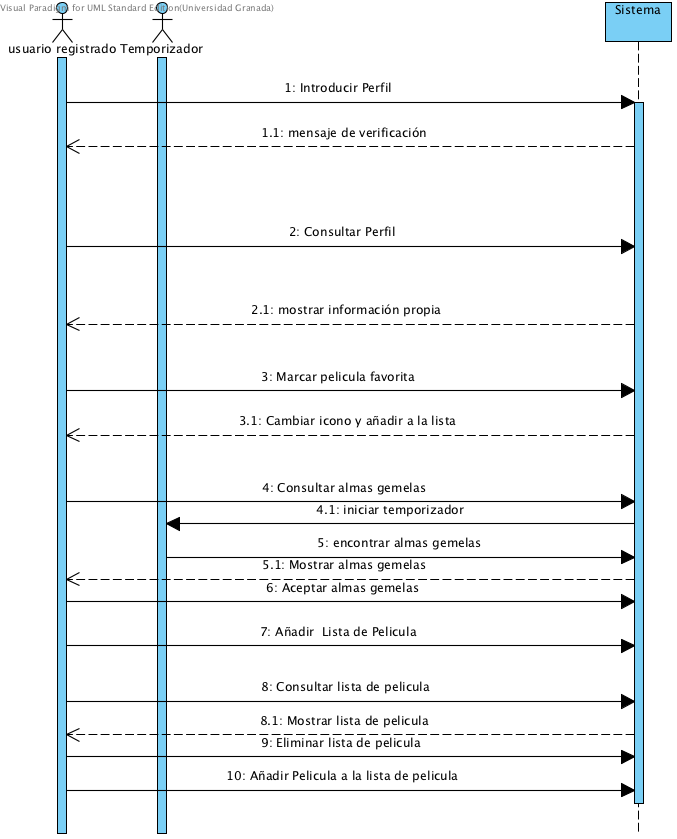
\includegraphics[width=1\linewidth]{./S-Perfil}
		
	\subsection*{Gestión de películas por usuarios. \textit{Jose Ramón Trillo Vilchez}}
	\begin{enumerate}
		\item El usuario puede buscar una película determinada.
    		\item El usuario puede consultar una cartelera en un cine determinado.
    		\item El usuario registrado puede puntuar una película.
    		\item Un usuario VIP puede añadir una película.
    		\item Un usuario VIP puede criticar una película determinada.
	\end{enumerate}
	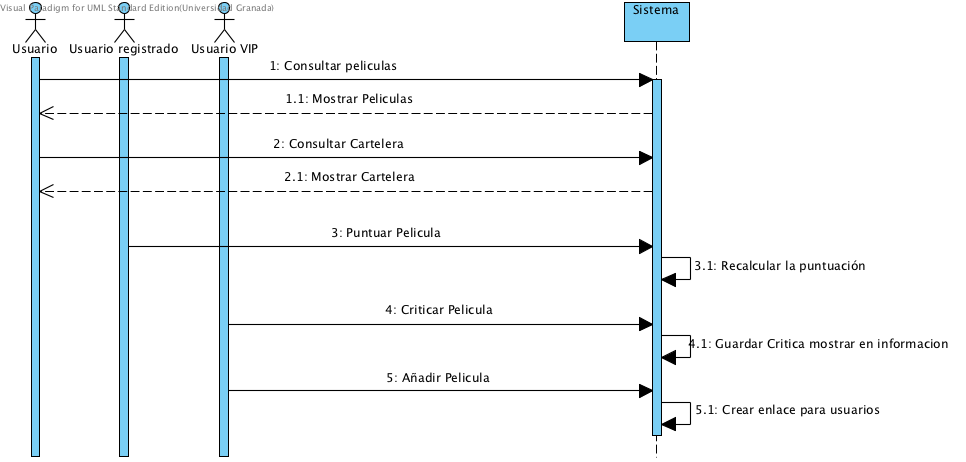
\includegraphics[width=1\linewidth]{./S-Peliculasusuarios}
		
	\subsection*{Gestión de comunidades. \textit{Lothar Soto Palma}}
	\begin{enumerate}
		\item El usuario registrado ingresa en el sistema.
		\item Se dirige al apartado dedicado a la gestión de comunidades.
		\item Crea una comunidad aunque para ello debe rellenar un formulario.
		\item El Usuario que quiere ser miembro de una comunidad solicita entrar en ella.
		\item El Usuario dueño admite o no al anterior usuario.
		\item La comunidad añade películas y las critica.
		\item El Usuario es capaz de listar las películas criticadas y añadidas por la comunidad.
	\end{enumerate}
		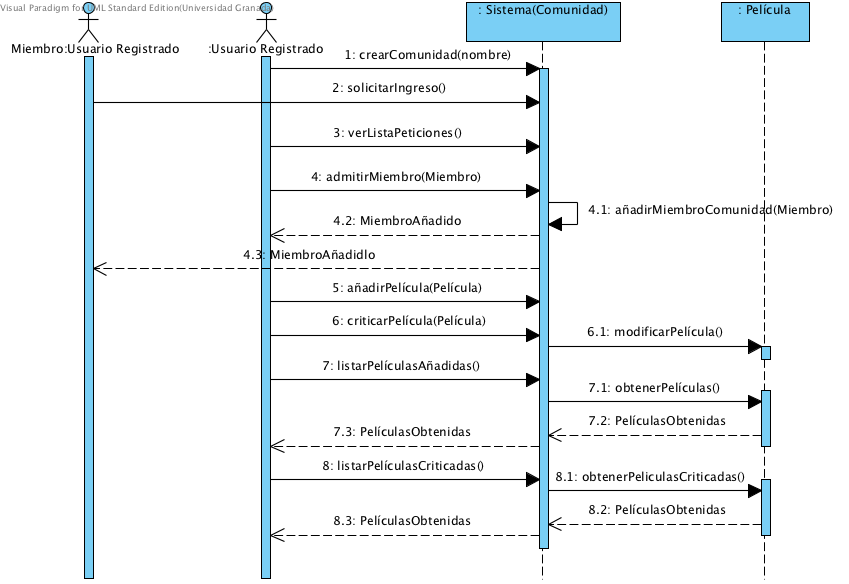
\includegraphics[width=1\linewidth]{./S-Comunidades}
\end{document}
